\documentclass{beamer}
\usepackage{graphicx, float}

\begin{document}
\title{Visualizing Multi-View Stereo}
\author{Andrew Morran, Ben Eysenbach}
\date{December 9, 2014}

\frame{\titlepage}

\section{Introduction}

\begin{frame}{Overview}
  \begin{center}
    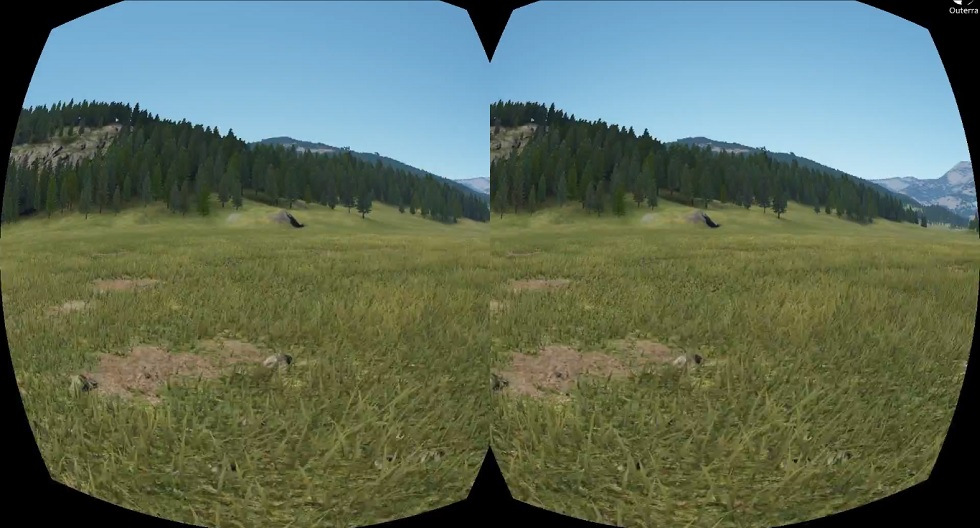
\includegraphics[width=0.5\textwidth]{rift.jpg}
  \end{center}

  Current technique for stereo reconstruction are complex. To help understand how different reconstruction pipelines work, we propose a novel visualization of the reconstruction process using an Oculus Rift. Given that stereo reconstruction is a series of manipulations on 3D data structures, it makes sense to be able to visualize the process in 3D.
\end{frame}


\begin{frame}{Overview}
  % one image per section
  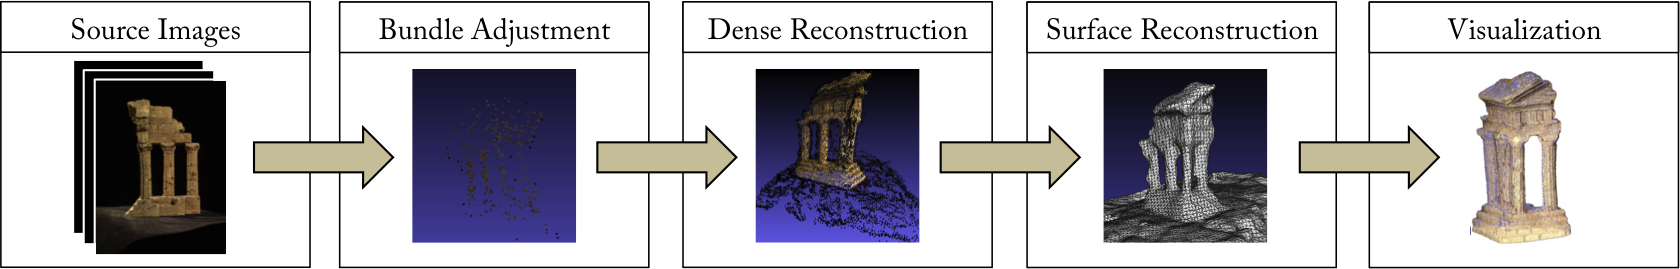
\includegraphics[width=\textwidth]{pipeline2.png}
  \tableofcontents  
\end{frame}

\section{Pose Estimation}

\begin{frame}{Bundle Adjustment and Sparse Reconstruction}
\end{frame}

\section{Dense Reconstruction}
\begin{frame}{Dense Reconstruction}
  PMVS
\end{frame}

\section{Surface Reconstruction}
\begin{frame}{Quadtrees}
  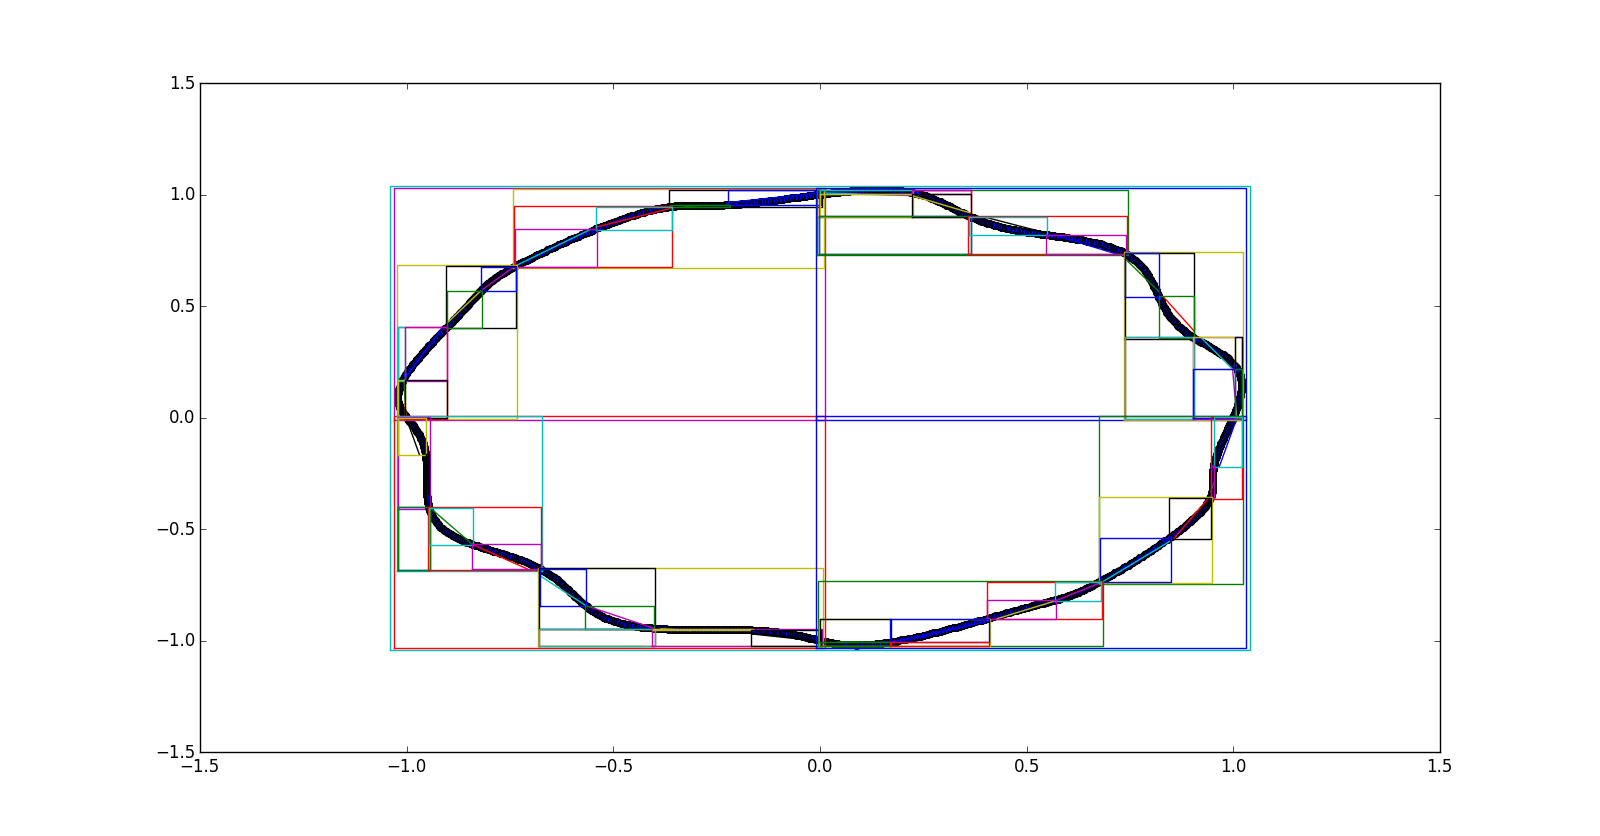
\includegraphics[width=\textwidth]{quadtree.png}
\end{frame}
\begin{frame}{Octrees}
  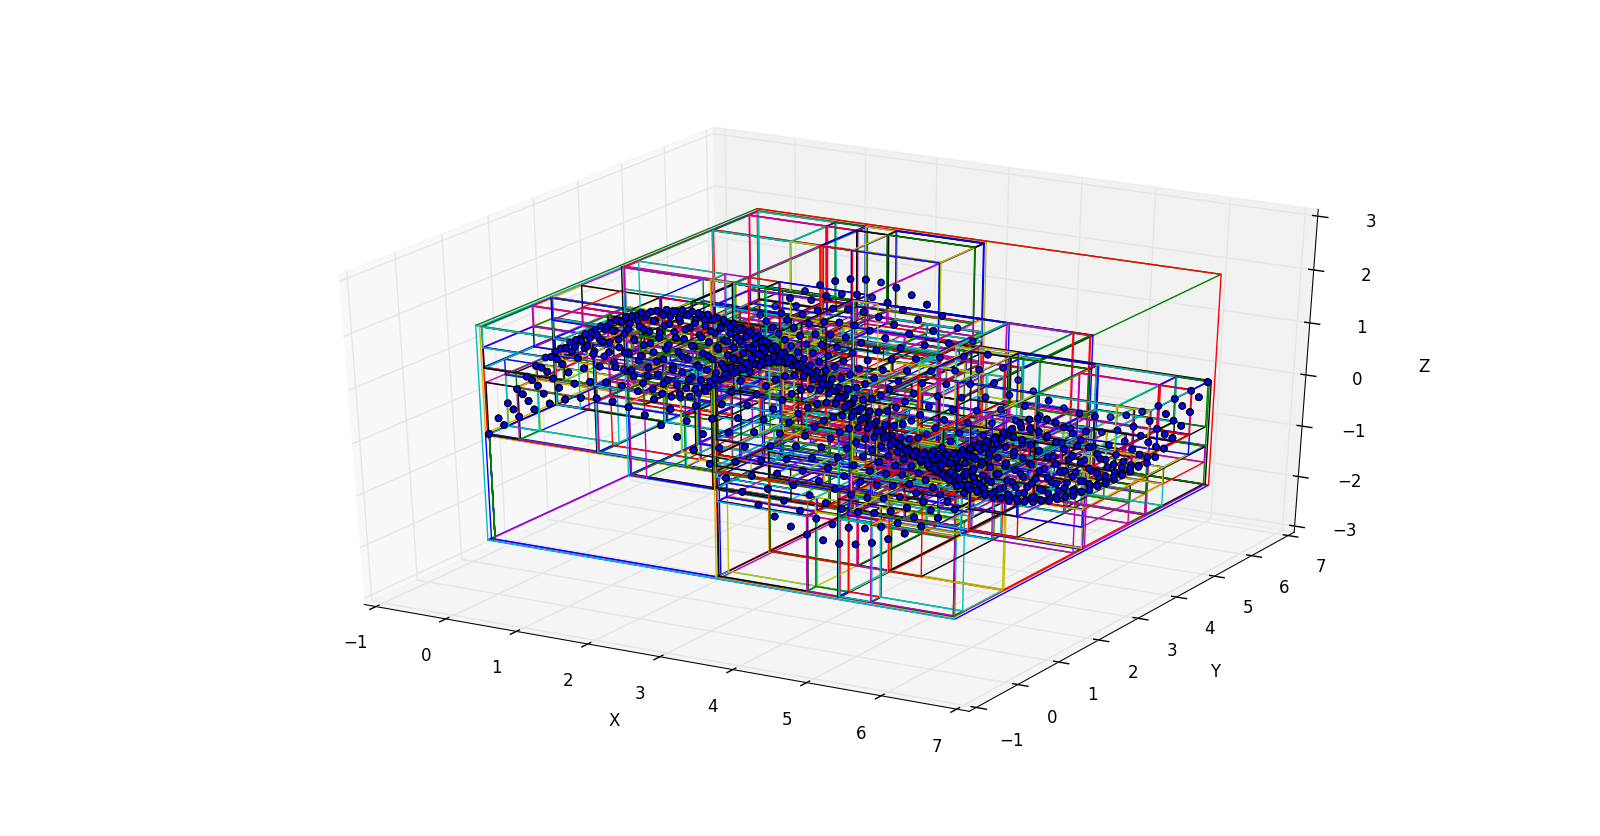
\includegraphics[width=\textwidth]{octree.png}
\end{frame}

\begin{frame}{Normal Estimation}
  % image of MST
\end{frame}

\begin{frame}{Constitent Normal Orientation}
\end{frame}

\begin{frame}{Signed Distance}
\end{frame}

\begin{frame}{Poisson Methods}
  % image of indicator function
\end{frame}

\begin{frame}{Marching Cubes}
  % image of marching squares
\end{frame}

\section{Conclusion}

\begin{frame}{Results}
  % Video of results}
\end{frame}

\begin{frame}{Thank You}
    % cool picture
\end{frame}

\begin{frame}{Questions?}
\end{frame}
  
\end{document}